
% \clearpage
% \KOMAoptions{paper=A3}
% % \addtolength{\textwidth}{1.35\textwidth}
% \recalctypearea

\newgeometry{margin=1.5cm}

\begin{landscape}
\thispagestyle{empty} %% Remove header and footer.

\begin{figure}
  \centering

  \begin{subfigure}[t]{0.49\textwidth}
    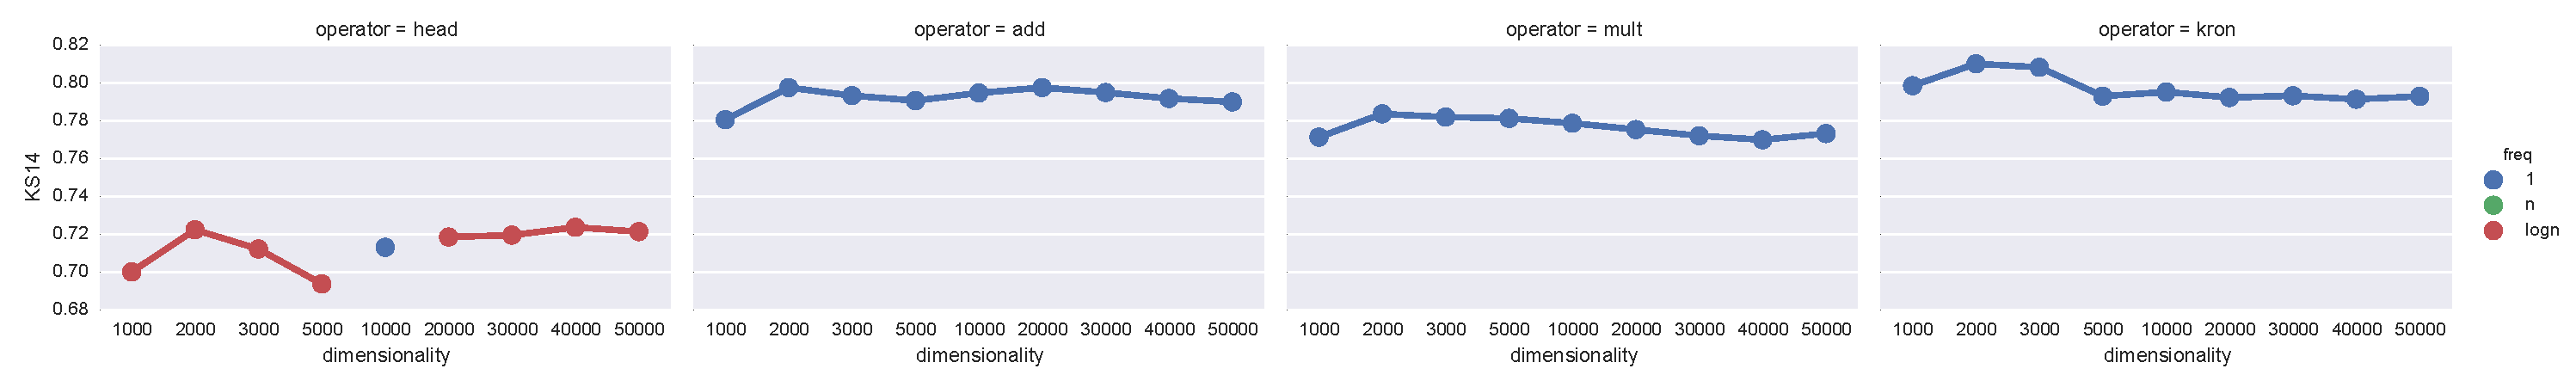
\includegraphics[width=\textwidth]{supplement/figures/KS14-max_-selection-freq}
    \caption{Max. Freq.}
    \label{fig:}
  \end{subfigure}
  \begin{subfigure}[t]{0.49\textwidth}
    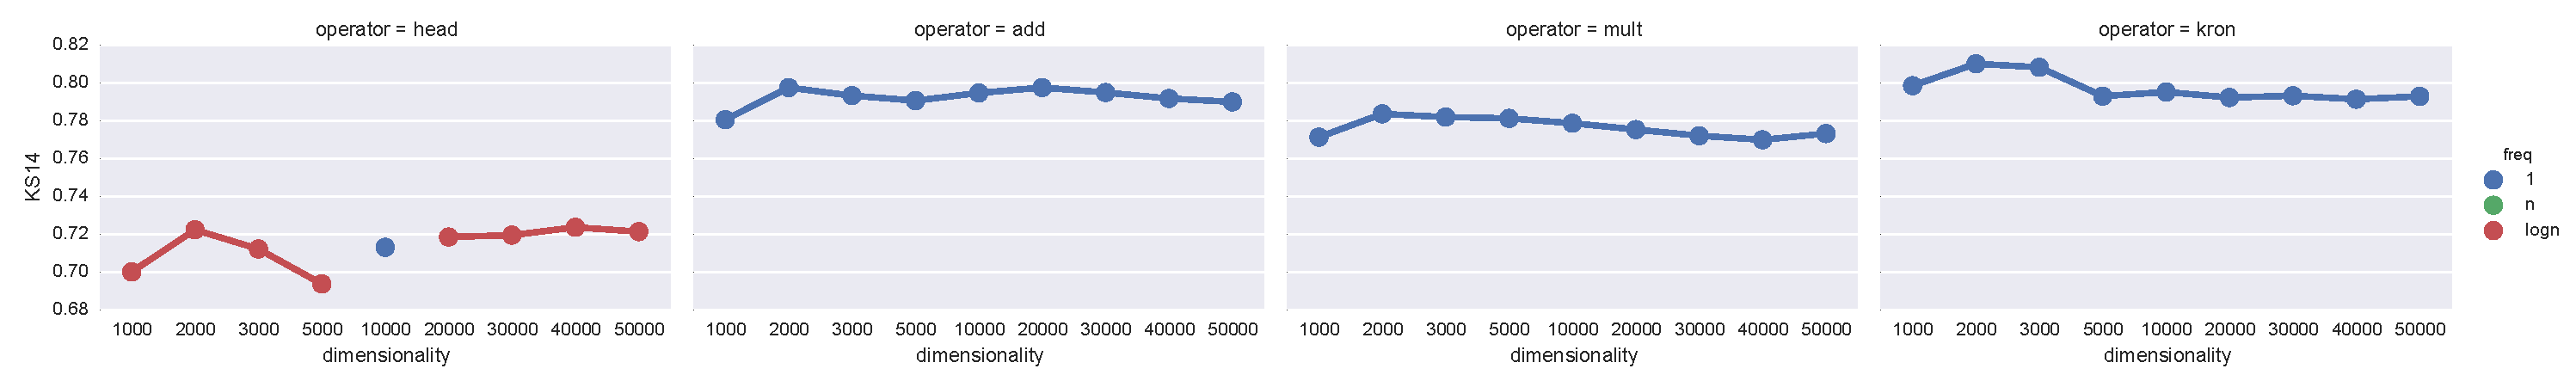
\includegraphics[width=\textwidth]{supplement/figures/KS14-cross_validation-selection-freq}
    \caption{CV. Freq.}
    \label{fig:}
  \end{subfigure}
  \begin{subfigure}[t]{0.49\textwidth}
    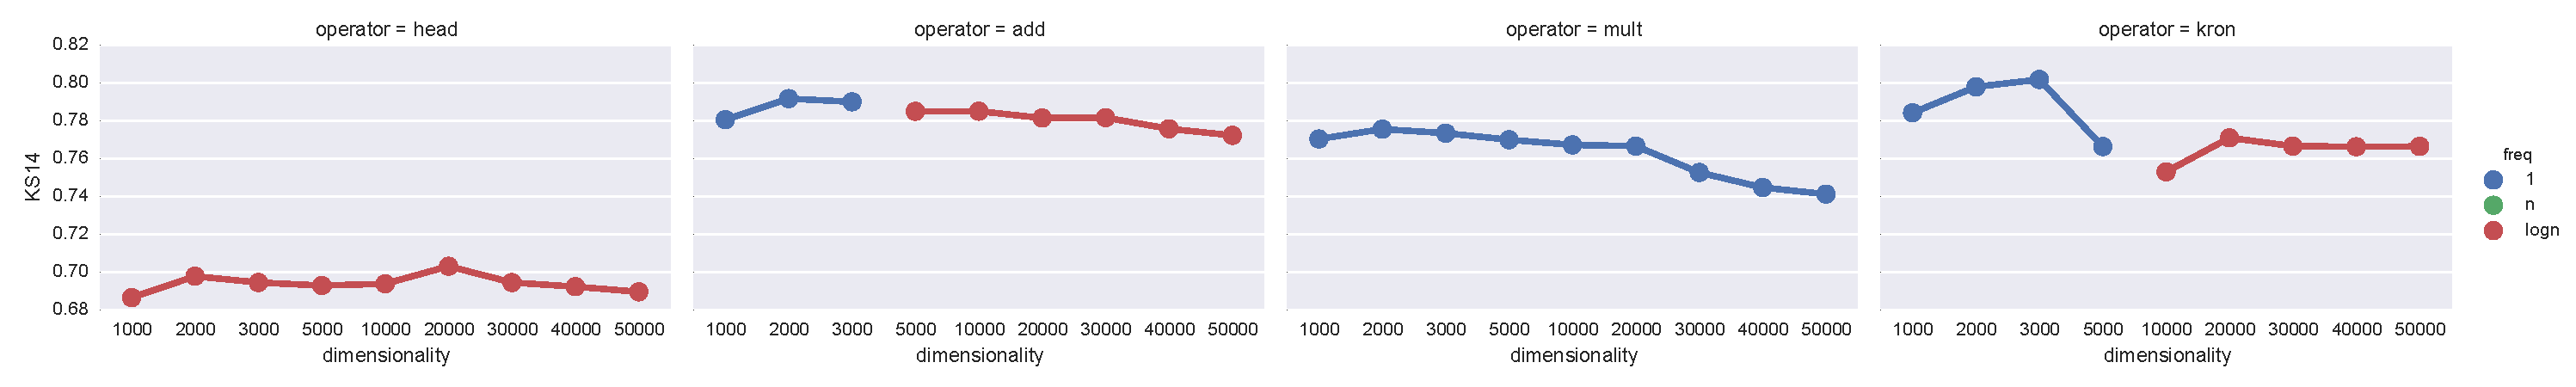
\includegraphics[width=\textwidth]{supplement/figures/KS14-heuristics-selection-freq}
    \caption{H. Freq.}
    \label{fig:}
  \end{subfigure}

  \begin{subfigure}[t]{0.49\textwidth}
    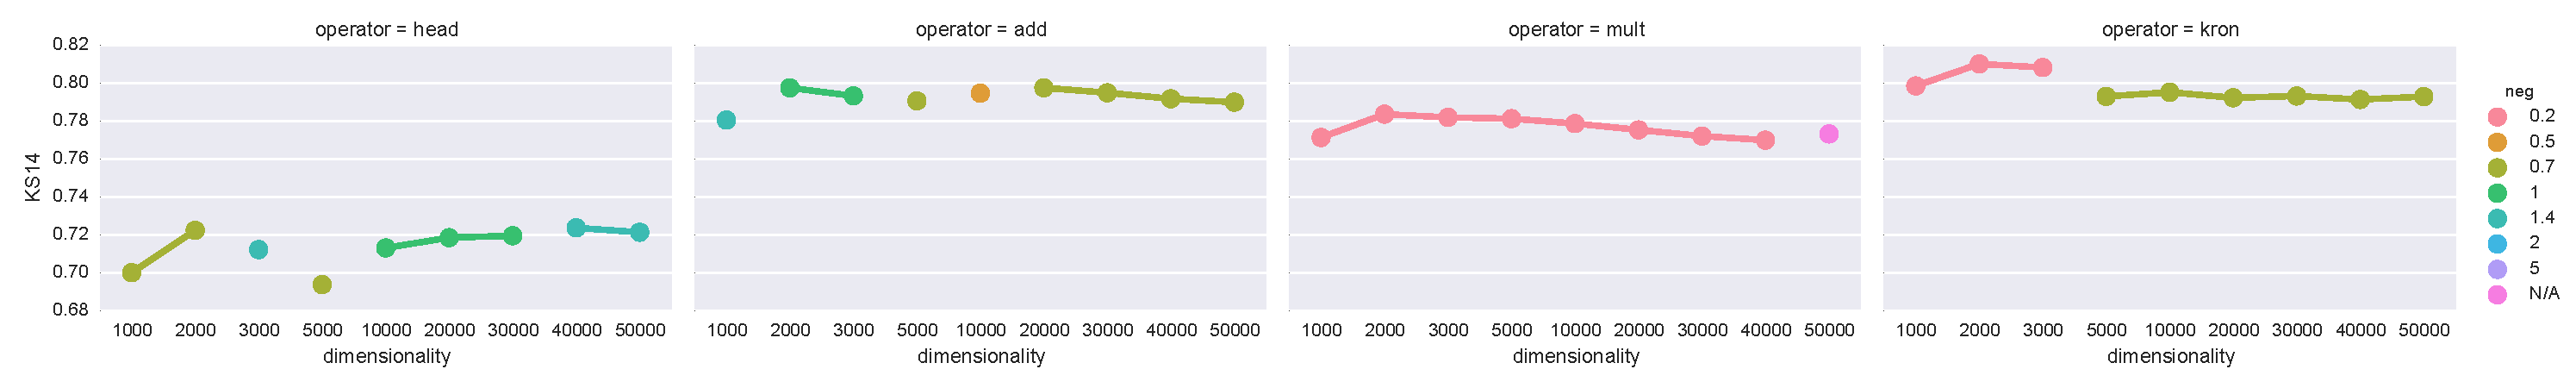
\includegraphics[width=\textwidth]{supplement/figures/KS14-max_-selection-neg}
    \caption{Max. Neg.}
    \label{fig:}
  \end{subfigure}
  \begin{subfigure}[t]{0.49\textwidth}
    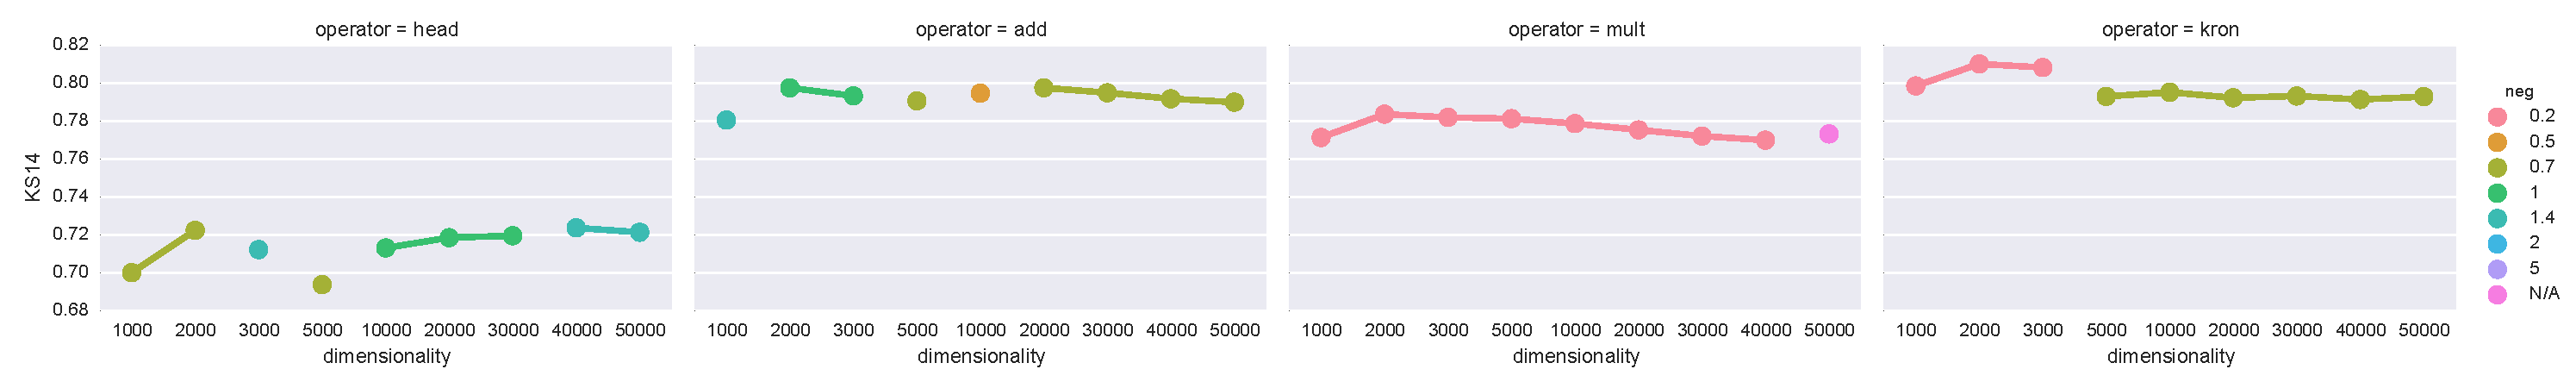
\includegraphics[width=\textwidth]{supplement/figures/KS14-cross_validation-selection-neg}
    \caption{CV. Neg.}
    \label{fig:}
  \end{subfigure}
  \begin{subfigure}[t]{0.49\textwidth}
    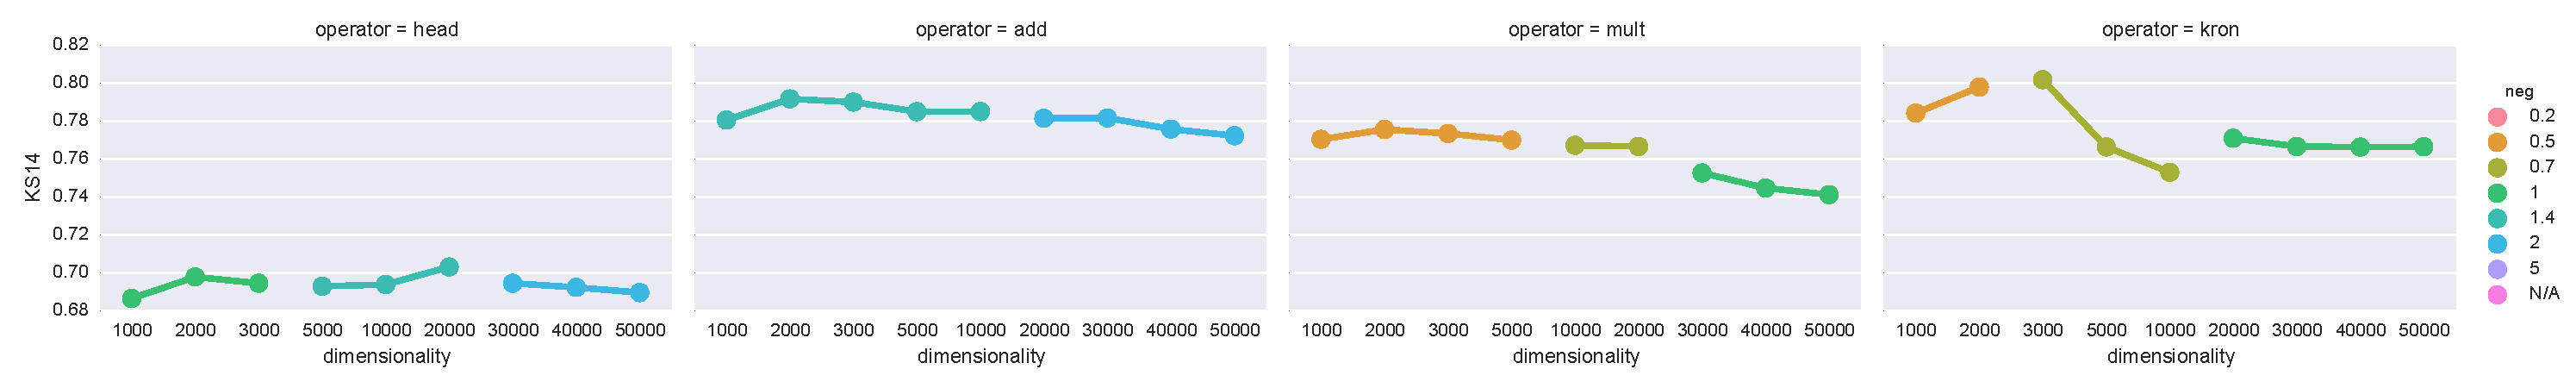
\includegraphics[width=\textwidth]{supplement/figures/KS14-heuristics-selection-neg}
    \caption{H. Neg.}
    \label{fig:}
  \end{subfigure}

  \begin{subfigure}[t]{0.49\textwidth}
    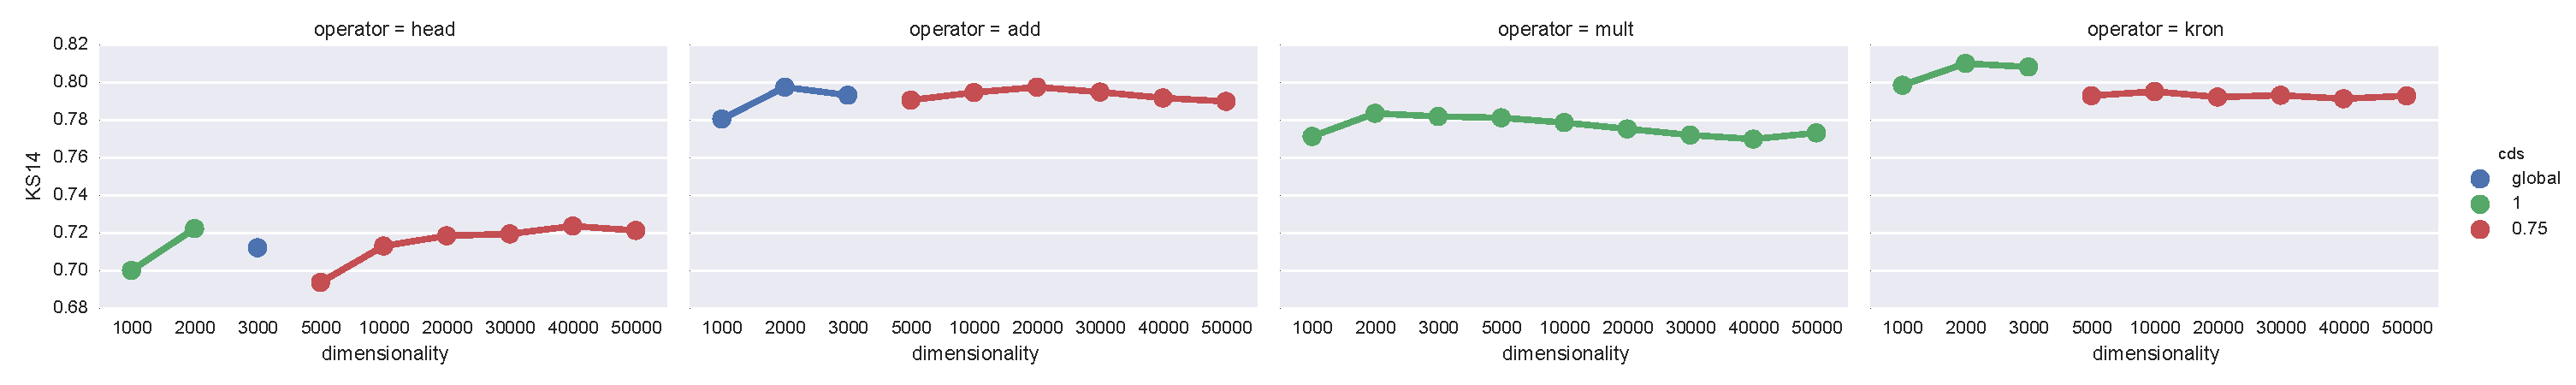
\includegraphics[width=\textwidth]{supplement/figures/KS14-max_-selection-cds}
    \caption{Max. CDS.}
    \label{fig:}
  \end{subfigure}
  \begin{subfigure}[t]{0.49\textwidth}
    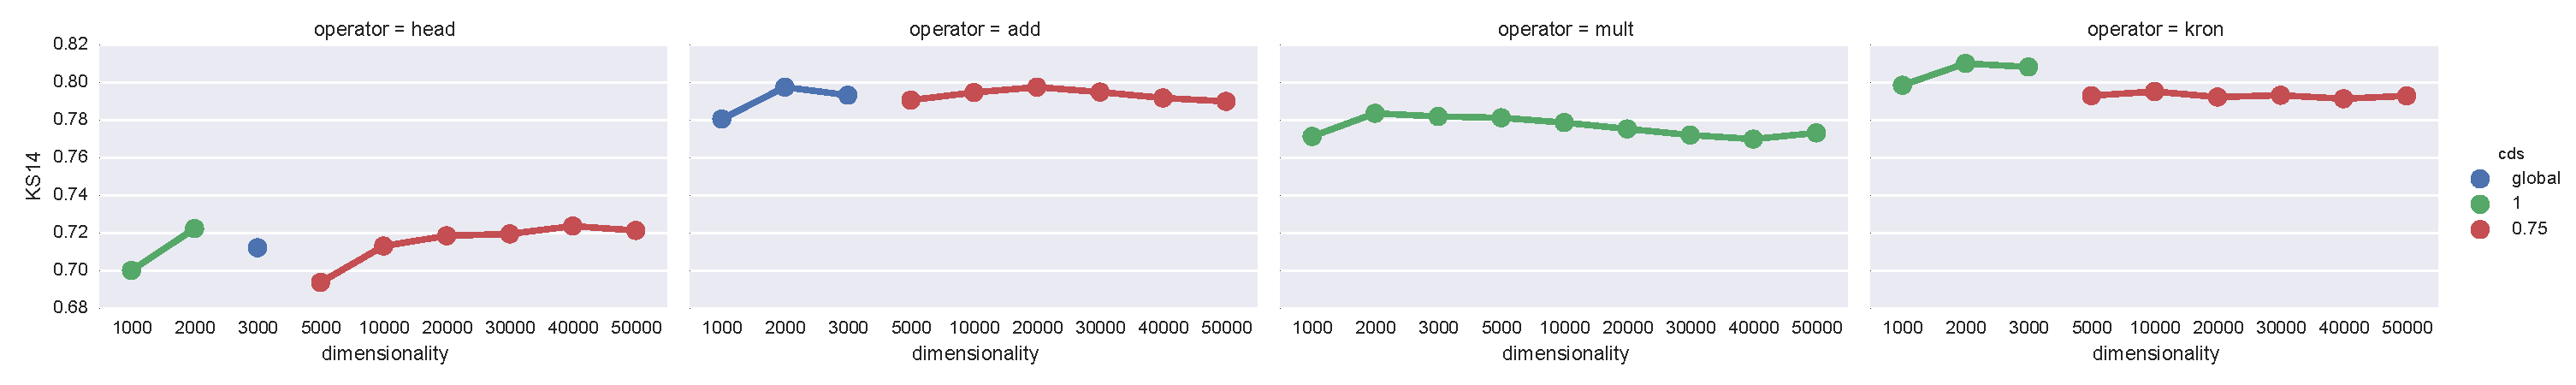
\includegraphics[width=\textwidth]{supplement/figures/KS14-cross_validation-selection-cds}
    \caption{CV. CDS.}
    \label{fig:}
  \end{subfigure}
  \begin{subfigure}[t]{0.49\textwidth}
    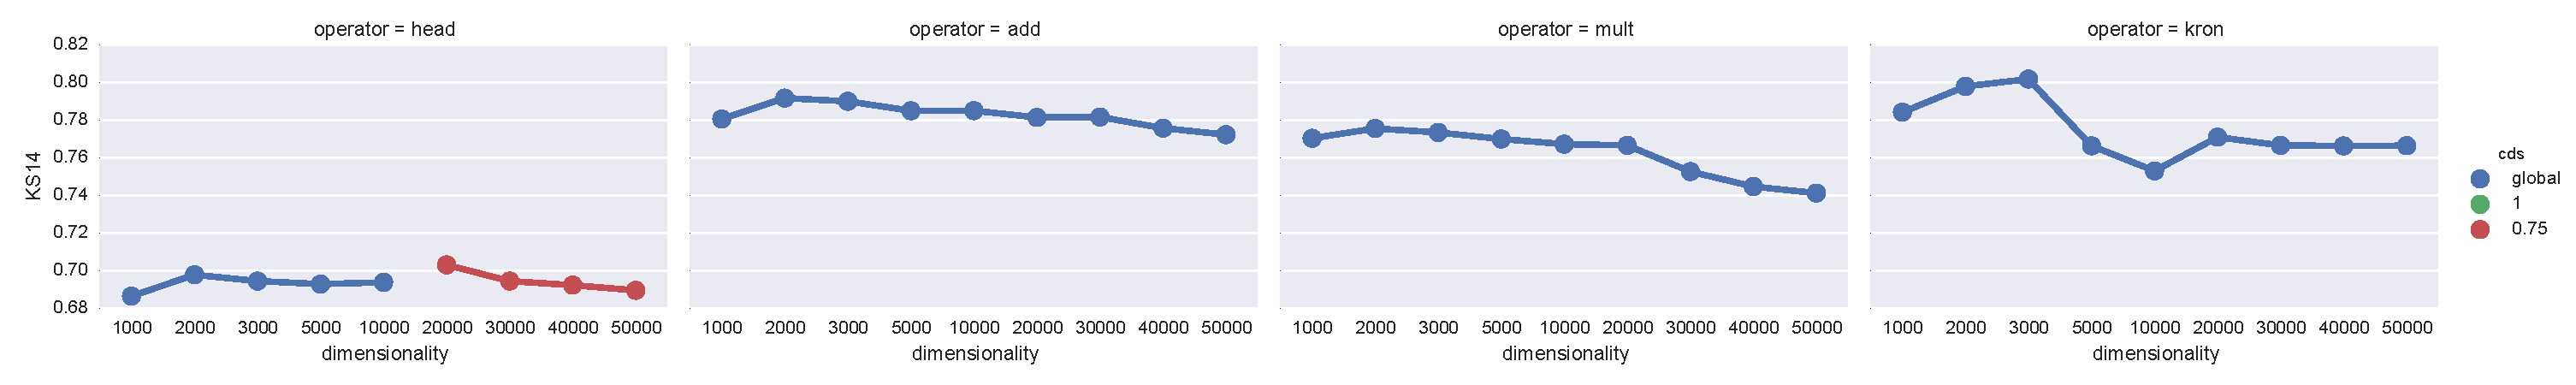
\includegraphics[width=\textwidth]{supplement/figures/KS14-heuristics-selection-cds}
    \caption{H. CDS.}
    \label{fig:}
  \end{subfigure}

  \begin{subfigure}[t]{0.49\textwidth}
    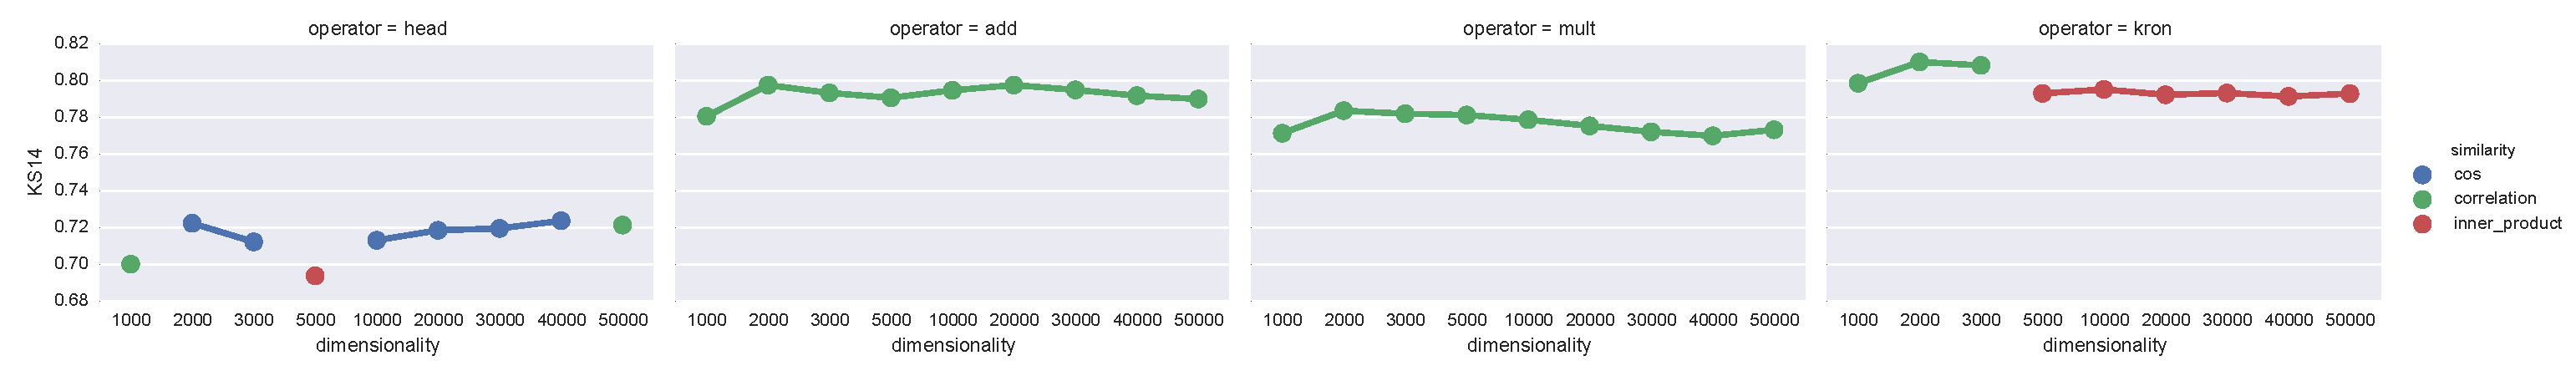
\includegraphics[width=\textwidth]{supplement/figures/KS14-max_-selection-similarity}
    \caption{Max. Sim.}
    \label{fig:}
  \end{subfigure}
  \begin{subfigure}[t]{0.49\textwidth}
    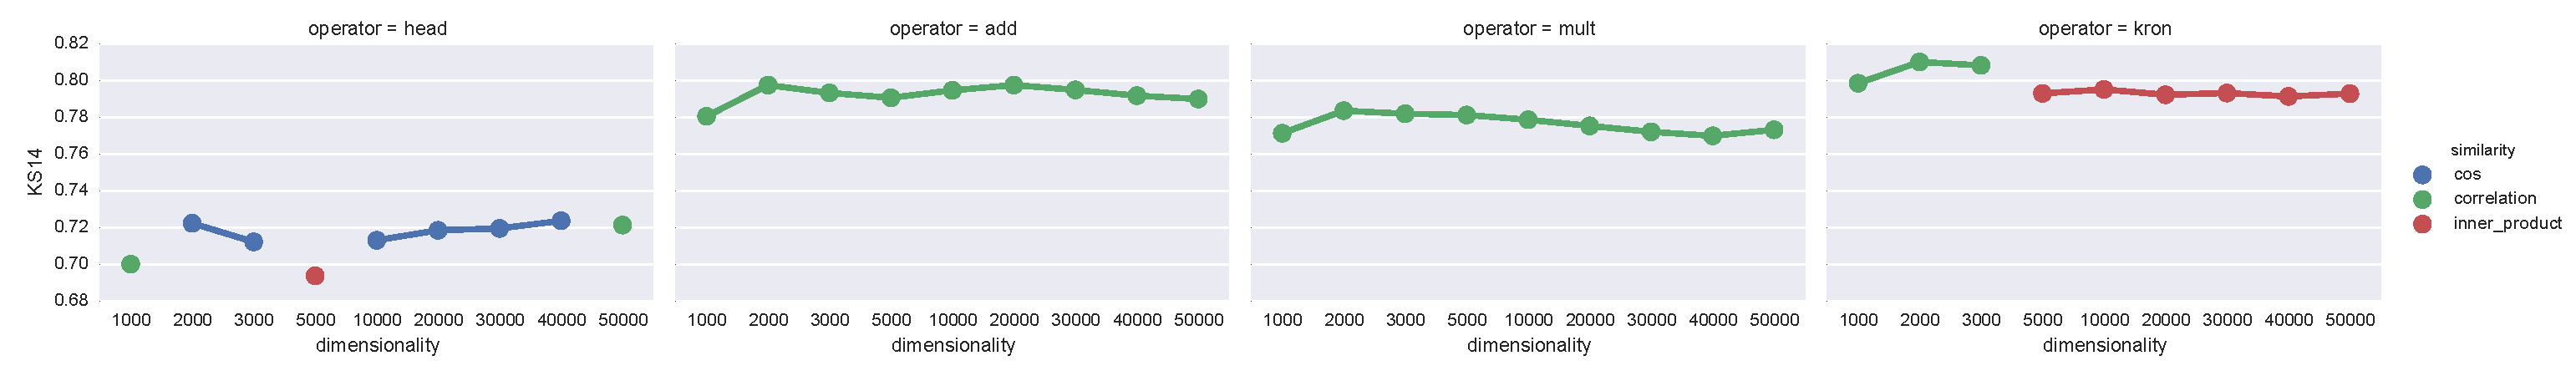
\includegraphics[width=\textwidth]{supplement/figures/KS14-cross_validation-selection-similarity}
    \caption{CV. Sim.}
    \label{fig:}
  \end{subfigure}
  \begin{subfigure}[t]{0.49\textwidth}
    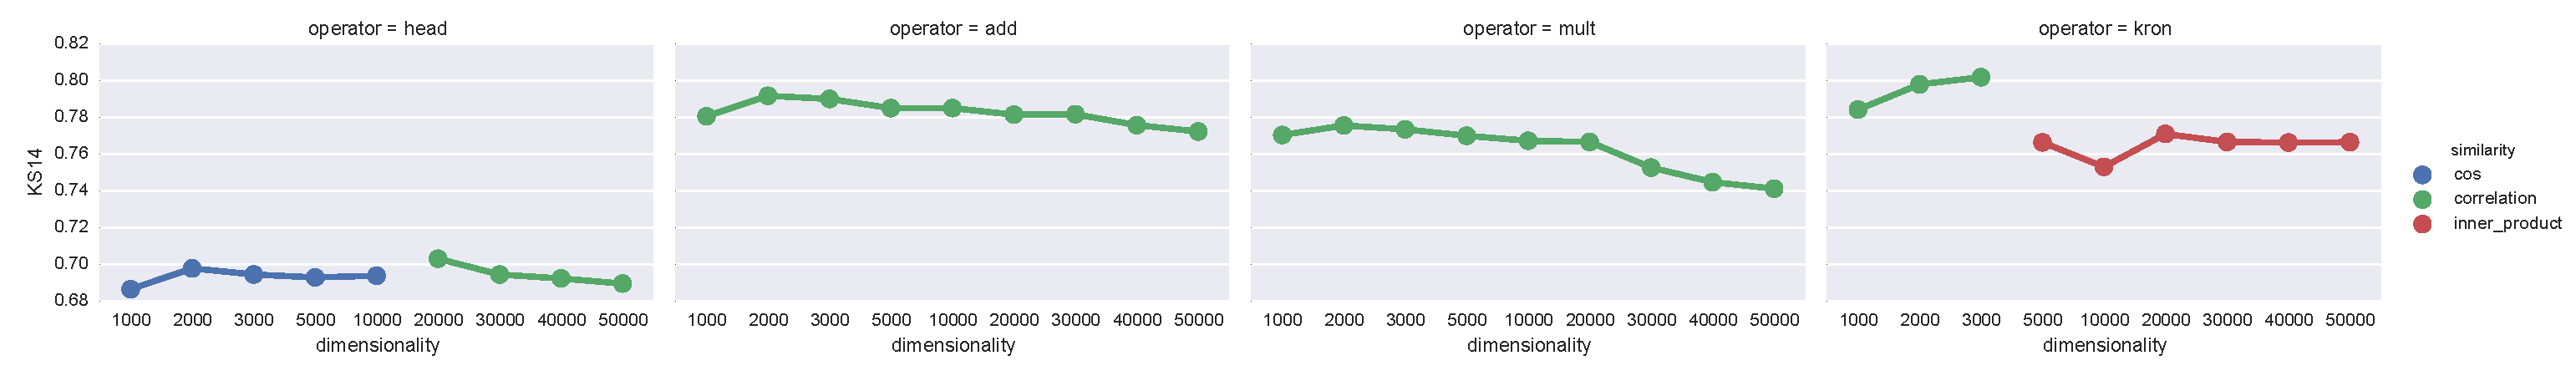
\includegraphics[width=\textwidth]{supplement/figures/KS14-heuristics-selection-similarity}
    \caption{H. Sim.}
    \label{fig:}
  \end{subfigure}

  \begin{subfigure}[t]{0.49\textwidth}
    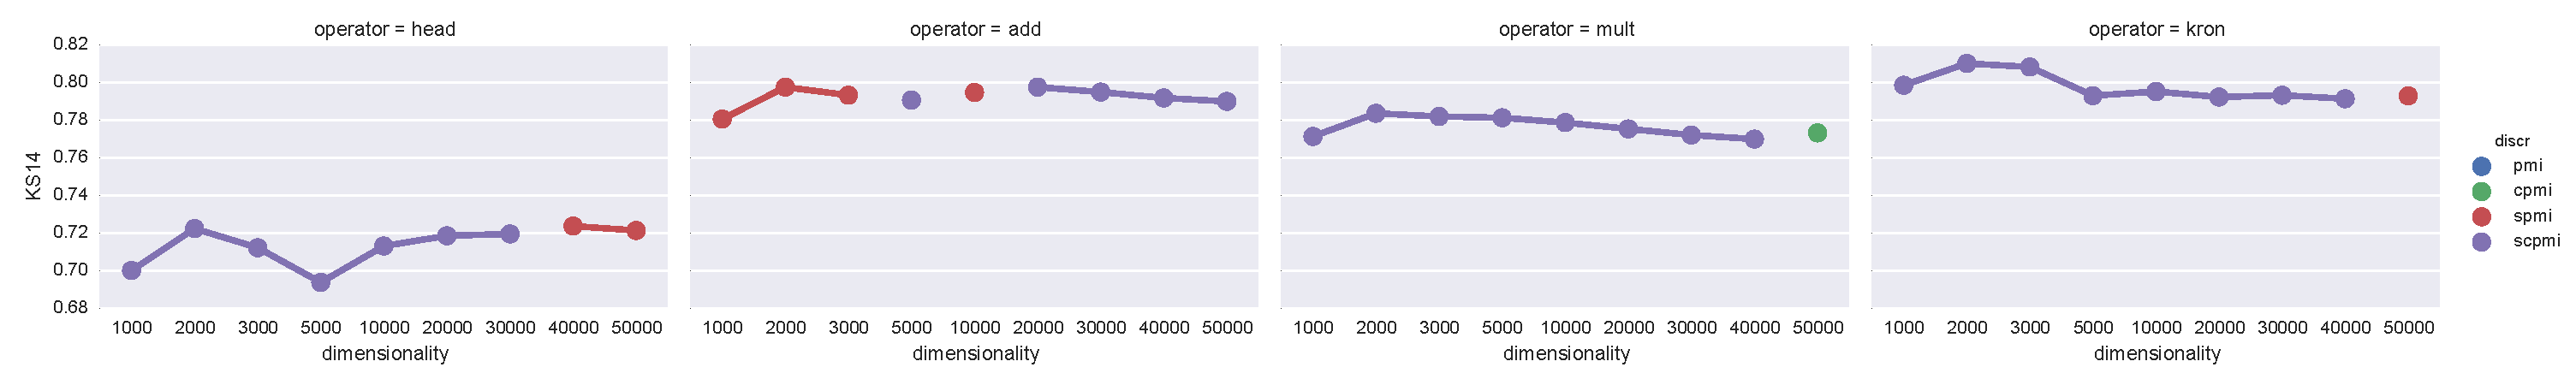
\includegraphics[width=\textwidth]{supplement/figures/KS14-max_-selection-discr}
    \caption{Max. Discr.}
    \label{fig:}
  \end{subfigure}
  \begin{subfigure}[t]{0.49\textwidth}
    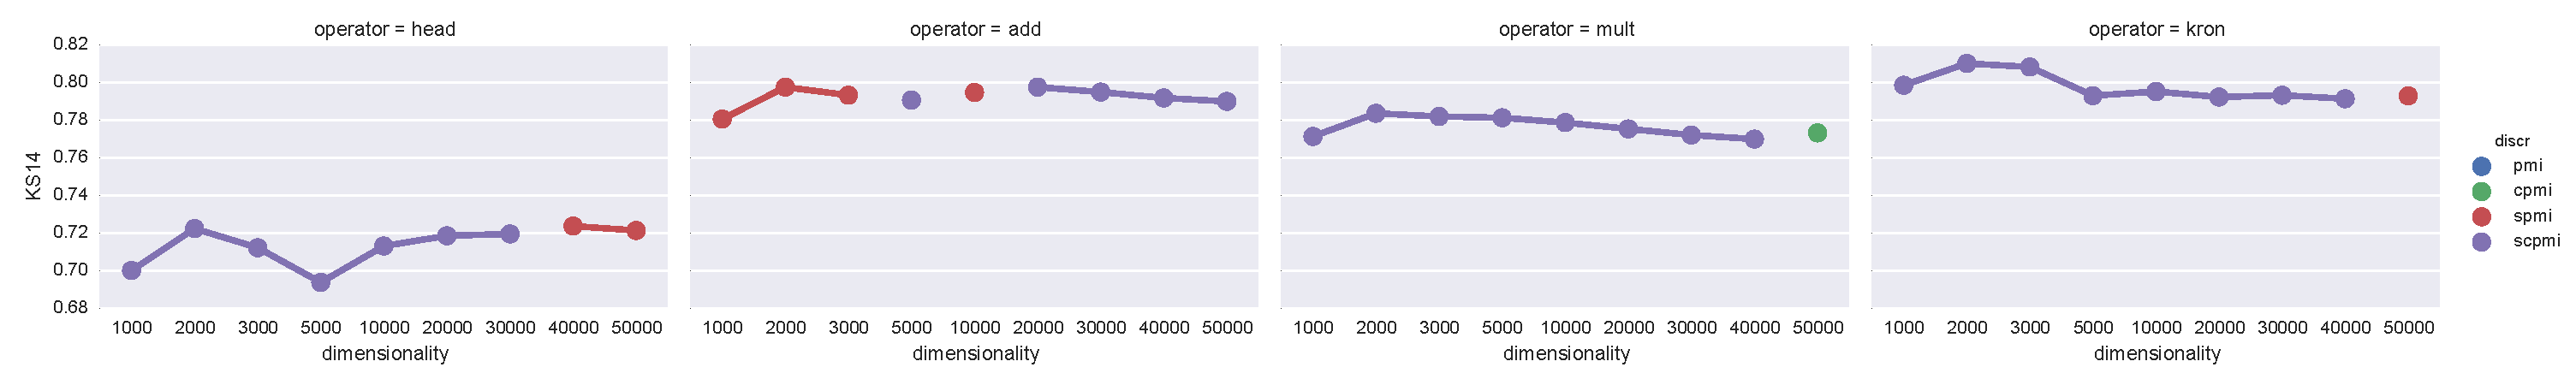
\includegraphics[width=\textwidth]{supplement/figures/KS14-cross_validation-selection-discr}
    \caption{CV. Discr.}
    \label{fig:}
  \end{subfigure}
  \begin{subfigure}[t]{0.49\textwidth}
    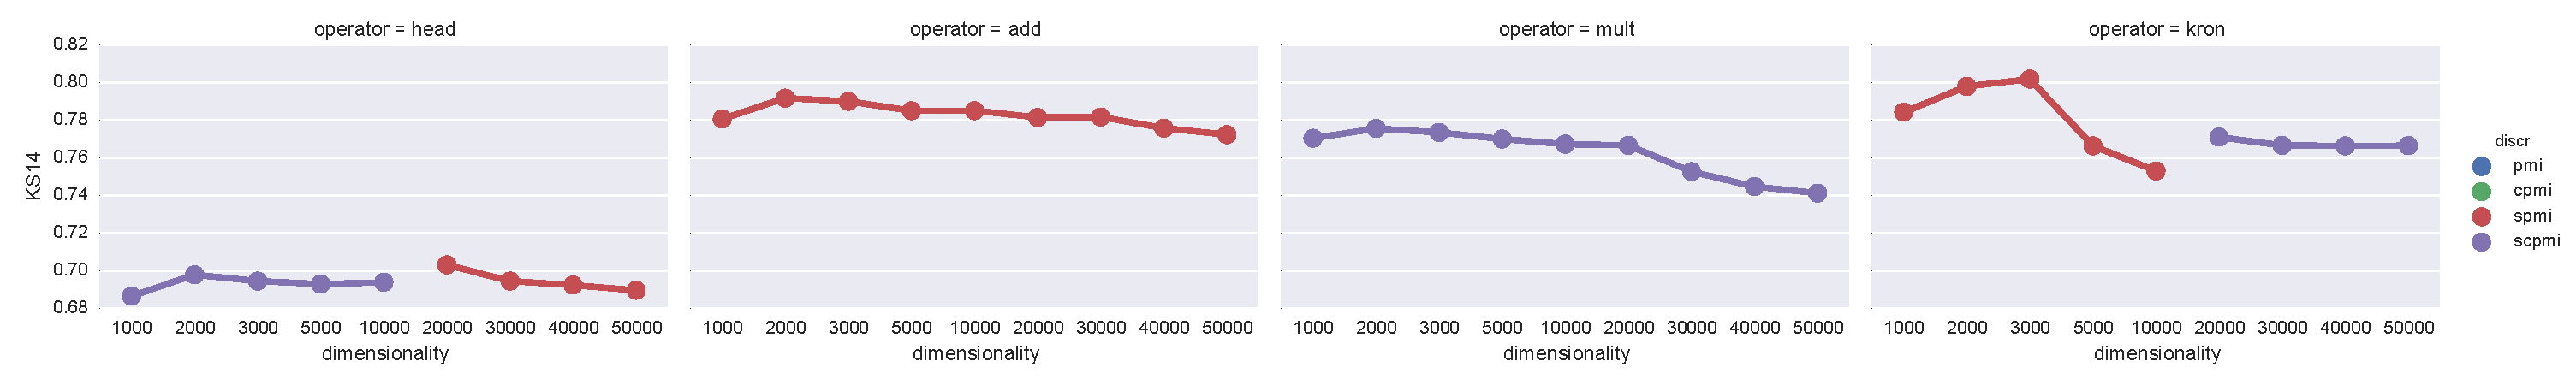
\includegraphics[width=\textwidth]{supplement/figures/KS14-heuristics-selection-discr}
    \caption{H. Discr.}
    \label{fig:}
  \end{subfigure}


  \caption{KS14 selection.}
  \label{fig:selection_ks14}
\end{figure}

\end{landscape}

\restoregeometry

% \clearpage
% \KOMAoptions{paper=A4,pagesize}
% \recalctypearea
